\begin{appendix}
\section{Anhang: Bestimmung der FWHM}
\begin{figure}[h]
\centering
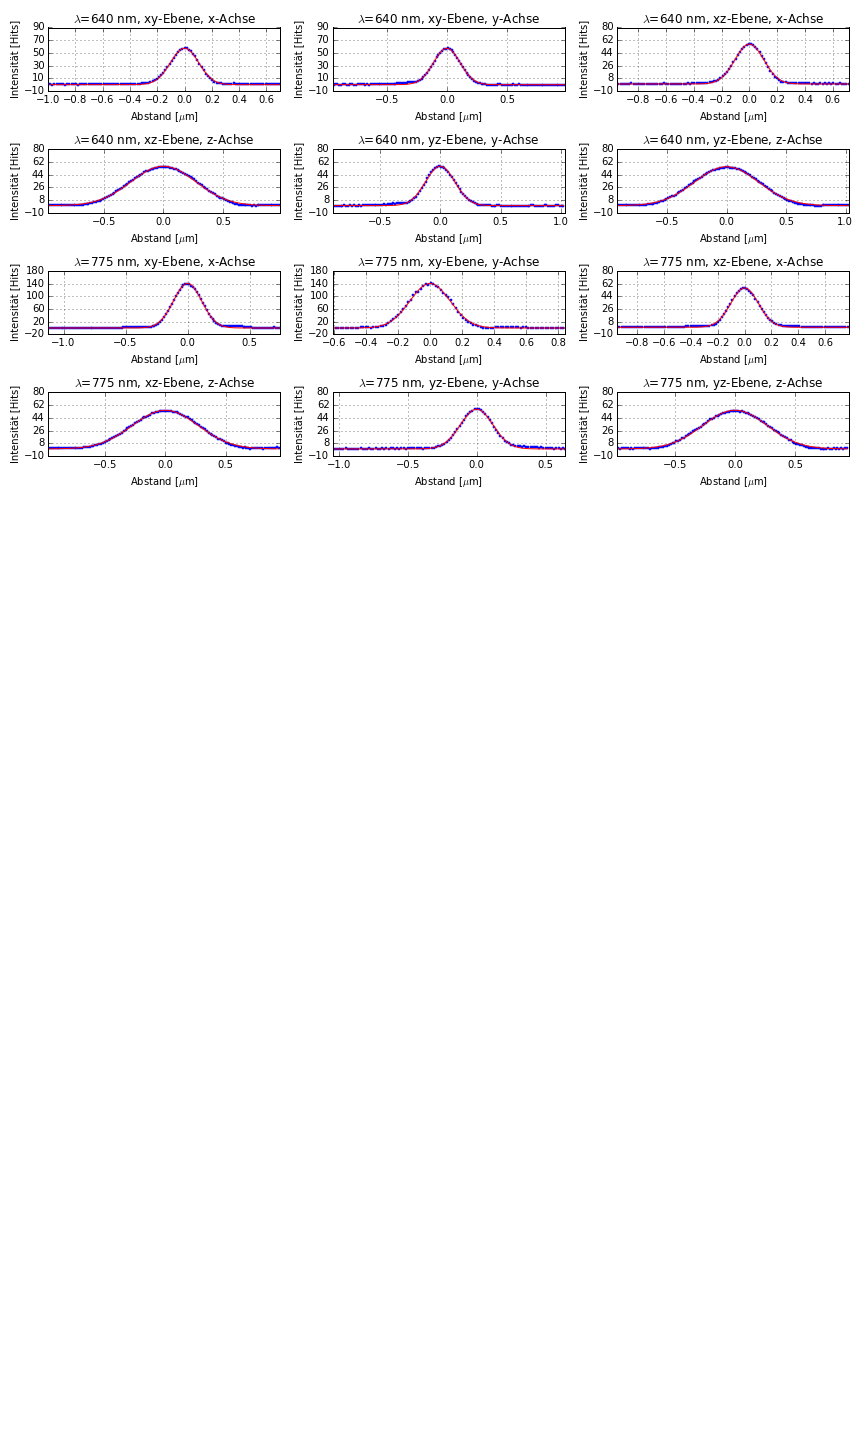
\includegraphics[trim= 0 950 0 0, width=\textwidth]{plots/goldbeads2.png}
\caption{Bestimmung der FWHM entlang aller Achsen für die Wellenlängen 640~nm und 775~nm. Die Intensitätsverläufe wurden mit einer Gauß'schen Funktion gefittet, um die Halbwertsbreite $\sqrt{2\log{2}}\sigma$ zu bestimmen.}\label{fig:gaussfits}
\end{figure}
\end{appendix}
